\مسئله{}
\پاسخ{}
\\
بخش ۱) vtable های مورد نظر به صورت زیر طراحی شده‌اند:
\graphicspath{{./images/}}
\begin{center}
	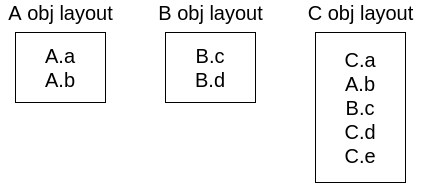
\includegraphics[scale=0.7]{q2_1.png}
\end{center}
در این بخش چون هیچ تابعی وجود ندارد، هیچ vtable ای نداریم و فقط ObjectLayout داریم. این ‌ها هم به سادگی قابل طراحی هستند، به این شکل که برای A و B که هیچ پدری ندارند صرفا field های خودشان را در layout می‌گذاریم و برای C که پدرانش A و B هستند، اجتماع field های هر ۳ کلاس را در نظر می‌گیریم. اگر هم که field ای هم در A (یا B ) و هم در C بود، طبیعتا آنی که در C است مدنظر گرفته می‌شود.
\\
\\
بخش ۲) vtable های مورد نظر به صورت زیر طراحی شده‌اند: (دقت فلش‌ها به این معنی است که آدرس خانه ته فلش در خانه سر آن ریخته شده است. مثلا آدرس شروع کد تابع f از کلاس A در خانه دوم از vtable مربوط به A ریخته شده است)
\begin{center}
	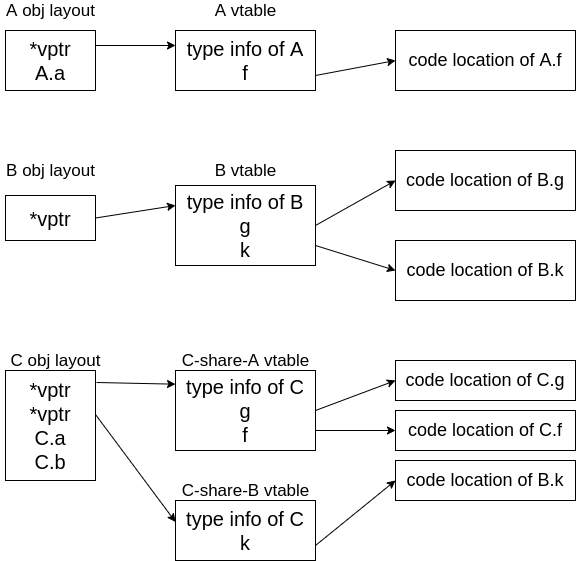
\includegraphics[scale=0.7]{q2_2.png}
\end{center}
در اینجا کلاس‌های A و B مانند بخش قبل طراحی می‌شوند، فقط چون تابع هم دارند باید vtable هم داشته باشند، البته چون هیچ‌یک پدری ندارند، طراحی vtable سخت نیست و مانند اسلایدها طراحی می‌شود. مثلا برای A آدرس کد تابع f در خانه دوم vtable آن ذخیره شده است. برای B هم به طور مشابه عمل شده است.
\\
اما برای کلاس C این‌گونه عمل می‌کنیم که ۲ تا vptr در obj layout شی C در نظر می‌گیریم. یکی به vtable ای اشاره می‌کند که توابعی را در خود دارد که یا در C هست و یا در A. 
vptr 
دومی به vtable ای اشاره می‌کند که در B هست ولی در C نیست. در واقع این دو vtable، یکی توابع A و یکی توابع B را دارد و در آن که توابع A وجود دارد، توابع C هم گنجاندیم. با این کار لازم نیست یک vptr سوم هم داشته باشیم و طراحی بهینه‌تر می‌شود. در نهایت این که خانه های درون vtable ها هم هرکدام به کد چه تابعی اشاره کند، مشخص شده است.
\\
\\
بخش ۳) vtable های مورد نظر به صورت زیر طراحی شده‌اند:
\begin{center}
	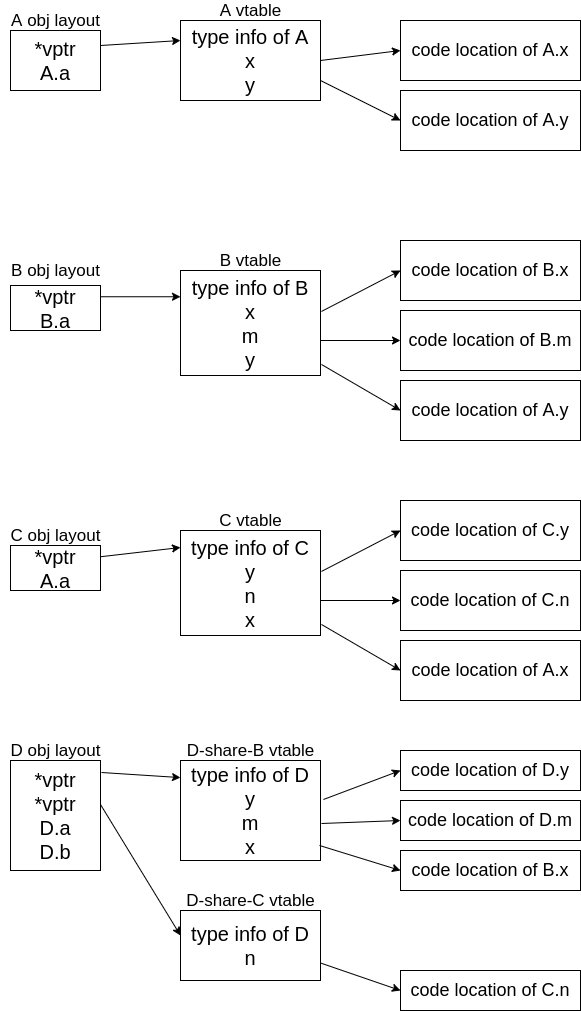
\includegraphics[scale=0.7]{q2_3.png}
\end{center}
vtable 
برای کلاس‌ A طراحی مانند بخش‌های قبل می‌شود. طراحی کلاس‌های B و C هم ساده است. کافی است مانند اسلایدهای درس این کار را انجام دهیم و برای هریک به تنها یک vtable نیاز داریم. اما در مورد D بحث کمی فرق می‌کند. اگر که تابعی در A تعریف شده باشد و B و C هم هردو آن را override کرده باشند، ولی در D override نشده باشد، به طور کلی زبان cpp توانایی تشخیص اینکه کدام یک را باید برای D در نظر گرفت ندارد و error می‌دهد. همچنین اگر تابع در C هم override نشده باشد، باز هم cpp خطا می‌دهد. مثل تابع x در اینجا که فقط در A و B تعریف شده است. در اینجا D نمی‌داند که باید x ای که در A آمده است را در نظر بگیرد یا آن که در B آمده است، چرا که اگر ارث‌بری کلاس‌ها را مانند درخت در نظر بگیریم، از D دو مسیر مختلف وجود دارد که در هر دو به کلاسی می‌رسیم که در آن x تعریف شده است. بنابراین تابع x مبهم خواهد بود.
\\
این مشکل را به این شکل در طراحی خودمان رفع کردیم که مثلا تابع تعریف شده در B را در نظر گرفتیم و نه آن که در A تعریف شده است. به عبارتی آنی را در نظر گرفتیم که در لایه‌های پایین‌تر است. بقیه طراحی مانند بخش‌های قبل است.






